% Taller 3 -- Punto 4: desarrollo propio (KMNIST) teniendo en cuenta la revisión del punto 3.   Compilar:  make punto4
% Las cifras (\cifra...) y las tablas salen de desarrollo/exportar_informe.py a partir del cuaderno ejecutado.
\documentclass[11pt,letterpaper]{article}
\usepackage{ud-informe}
% Acento azul: el logo del programa (MCIC) es azul, así que se usa la gama azur del manual de marca en lugar del rojo.
% Para volver al rojo institucional de la plantilla, borrar estas dos líneas.
\colorlet{udrojo}{udazul}
\definecolor{udrojoosc}{HTML}{0C6F96}
% Generado por desarrollo/exportar_informe.py: NO editar a mano.
\newcommand{\cifraaugLoteVal}{0,00}
\newcommand{\cifraaugLoteValGana}{1}
\newcommand{\cifraaugLoteTe}{$-$0,33}
\newcommand{\cifraaugLoteTeGana}{1}
\newcommand{\cifraaugMuestraVal}{0,12}
\newcommand{\cifraaugMuestraValGana}{3}
\newcommand{\cifraaugMuestraTe}{$-$0,25}
\newcommand{\cifraaugMuestraTeGana}{1}
\newcommand{\cifraaugN}{5}
\newcommand{\cifralargoValDif}{$-$0,15}
\newcommand{\cifralargoTeDif}{$-$0,19}
\newcommand{\cifralargoBrechaSin}{1,09}
\newcommand{\cifralargoBrechaCon}{0,40}
\newcommand{\cifraablBnTe}{0,54}
\newcommand{\cifraablBnVal}{0,32}
\newcommand{\cifraablBnBrecha}{0,83}
\newcommand{\cifraablDropTe}{$-$0,52}
\newcommand{\cifraablDropVal}{$-$0,47}
\newcommand{\cifraablDropBrecha}{1,45}
\newcommand{\cifraablAmbosTe}{0,46}
\newcommand{\cifraablAmbosVal}{0,11}
\newcommand{\cifraablAmbosBrecha}{1,46}
\newcommand{\cifraablTresTe}{2,11}
\newcommand{\cifraablTresVal}{1,07}
\newcommand{\cifraablTresBrecha}{0,89}
\newcommand{\cifraablBrechaCompleta}{0,90}
\newcommand{\ciframlpTe}{88,44}
\newcommand{\cifracnnDocTe}{91,20}
\newcommand{\cifracnnPropTe}{92,10}
\newcommand{\cifracnnPropVsMlp}{3,66}
\newcommand{\cifracnnPropVsDoc}{0,90}
\newcommand{\cifradsMNISTTe}{98,80}
\newcommand{\cifradsMNISTVal}{98,72}
\newcommand{\cifradsMNISTGap}{$-$0,1}
\newcommand{\cifradsMNISTPeor}{97,2}
\newcommand{\cifradsMNISTBajo}{0,0}
\newcommand{\cifradsFashionMNISTTe}{90,27}
\newcommand{\cifradsFashionMNISTVal}{90,34}
\newcommand{\cifradsFashionMNISTGap}{0,1}
\newcommand{\cifradsFashionMNISTPeor}{72,2}
\newcommand{\cifradsFashionMNISTBajo}{4,3}
\newcommand{\cifradsKMNISTTe}{92,10}
\newcommand{\cifradsKMNISTVal}{97,15}
\newcommand{\cifradsKMNISTGap}{5,1}
\newcommand{\cifradsKMNISTPeor}{86,3}
\newcommand{\cifradsKMNISTBajo}{2,0}
\newcommand{\cifralrUno}{82,46}
\newcommand{\cifralrSinBnUno}{9,76}
\newcommand{\cifralrDos}{96,70}
\newcommand{\cifralrSinBnDos}{92,62}
\newcommand{\cifralrTres}{96,30}
\newcommand{\cifralrSinBnTres}{96,52}
\newcommand{\cifralrCuatro}{92,38}
\newcommand{\cifralrCinco}{76,30}
\newcommand{\cifraaccTest}{91,85}
\newcommand{\cifraaccVal}{97,40}
\newcommand{\cifraaccTr}{96,31}
\newcommand{\cifraerrTest}{815}
\newcommand{\cifralossIni}{0,374}
\newcommand{\cifralossFin}{0,117}
\newcommand{\cifraepocas}{5}
\newcommand{\cifraparA}{su}
\newcommand{\cifraparB}{tsu}
\newcommand{\cifraparN}{60}
\newcommand{\cifraparInv}{21}
\newcommand{\cifraclaseMejor}{tsu}
\newcommand{\cifraclaseMejorAcc}{96,5}
\newcommand{\cifraclasePeor}{su}
\newcommand{\cifraclasePeorAcc}{82,2}
\newcommand{\cifrabrechaValTest}{5,5}


\newcommand{\pts}{\,pts}

\renewcommand{\UDtitulo}{Desarrollo propio con KMNIST}
\renewcommand{\UDsubtitulo}{CNN en PyTorch teniendo en cuenta la revisión del script del profesor}
\renewcommand{\UDtipo}{Taller 3 -- Punto 4 -- Informe de ejecución}
\renewcommand{\UDasignatura}{Inteligencia Computacional Aplicada}
\renewcommand{\UDdocente}{Cesar Andrey Perdomo Charry}
\renewcommand{\UDestudiantes}{Juan Felipe Rodríguez Galindo -- 20261595004}
\renewcommand{\UDencabezado}{Taller 3 -- Punto 4: desarrollo propio}

\begin{document}
\UDportada

%% ---------------------------------------------------------------------------------------------
\section{Qué se hizo y cómo se relaciona con el punto 3}

Se repitió el flujo del cuaderno del profesor con \textbf{KMNIST} (70\,000 imágenes de $28\times28$ de hiragana cursivo, 10 clases), se completaron los cinco bloques \texttt{TODO}
del cuaderno propuesto y se respondieron sus tres preguntas. La revisión del punto 3 se usó como guía: la tabla~\ref{tab:rel} indica qué se conservó y qué se cambió o agregó.

\begin{table}[H]
\centering\small
\caption{Qué se conservó del script y qué se cambió o agregó.}\label{tab:rel}
\begin{tabularx}{\linewidth}{@{}l L L@{}}
\toprule
Decisión & Según la revisión del script (punto 3) & Qué se hizo en el desarrollo propio \\
\midrule
Conservado & Partición 55\,000 / 5\,000 / 10\,000, normalización solo con estadísticos del entrenamiento, prueba usada una vez & Igual; la prueba solo informa el resultado final \\
Conservado & Puntos de control \texttt{verificar()}, Adam con $\eta=10^{-3}$, lotes de 64 & Igual: 11 verificaciones del taller y 9 propias \\
Cambiado & CNN sin relleno ni \textit{BatchNorm} (12\,810 parámetros) & \texttt{CNNPropia}: relleno 1, \textit{BatchNorm} y \textit{dropout} 0,3; \textbf{20\,586} parámetros \\
Cambiado & Comparaciones no pareadas, una sola corrida & Cargador de datos por corrida y \textbf{5 semillas} (aumento) o 3 (ablación y bases) \\
Cambiado & Paso 5 con 3 tasas, 2 épocas y sin control & 5 tasas de $10^{-1}$ a $10^{-5}$ y un control sin \textit{BatchNorm} \\
Cambiado & MLP no evaluado en prueba & MLP y CNN del docente evaluados en prueba (\ciframlpTe\,\% y \cifracnnDocTe\,\%) \\
Cambiado & Solo MNIST & KMNIST como conjunto principal; FashionMNIST y MNIST con la misma red \\
\bottomrule
\end{tabularx}
\end{table}

%% ---------------------------------------------------------------------------------------------
\section{Ejecución}

El cuaderno \texttt{Taller\_3\_CNN\_KMNIST.ipynb} se ejecutó \textbf{de principio a fin, sin errores}, con las salidas visibles, en CPU (Apple M1, PyTorch 2.14.1). Cada bloque del taller
termina en un punto de control automático; los 11 del taller y 9 propios pasaron (\texttt{[OK]}).

\begin{figure}[H]
\centering
\begin{tikzpicture}[node distance=0.28cm]
  \node[caja] (e0) {\textbf{Paso 0}\\\footnotesize entorno};
  \node[caja, right=of e0] (e1) {\textbf{TODO 1}\\\footnotesize datos};
  \node[caja, right=of e1] (e2) {\textbf{TODO 2}\\\footnotesize \texttt{CNNPropia}};
  \node[caja, right=of e2] (e3) {\textbf{TODO 3}\\\footnotesize entrenar};
  \node[caja, right=of e3] (e4) {\textbf{TODO 4}\\\footnotesize prueba};
  \node[hecho, right=of e4] (e5) {\textbf{TODO 5}\\\footnotesize aumento};
  \foreach \i/\j in {e0/e1,e1/e2,e2/e3,e3/e4,e4/e5} \draw[flecha] (\i) -- (\j);
\end{tikzpicture}
\caption{Bloques ejecutados; todos pasaron su punto de control.}
\end{figure}

\begin{table}[H]
\centering\small
\caption{Puntos de control del cuaderno. Los 11 primeros son los del taller; además hay 9 verificaciones propias.}
\begin{tabularx}{\linewidth}{@{}l L l l@{}}
\toprule
Bloque & Verificación & Valor observado & Estado \\
\midrule
TODO 1 & El conteo por clase suma las imágenes de entrenamiento & 55\,000 (razón máx/mín 1,015) & OK \\
TODO 2 & Salida de forma $(4,10)$ & $(4,10)$ & OK \\
       & Menos de 200\,000 parámetros & 20\,586 & OK \\
       & Usa \texttt{BatchNorm2d} y \texttt{Dropout} & ambos presentes & OK \\
       & Al menos 2 capas convolucionales & 2 & OK \\
TODO 3 & La pérdida de entrenamiento baja entre la primera y la última época & \cifralossIni{} $\to$ \cifralossFin & OK \\
       & Exactitud de validación $>$ 80\,\% & \cifraaccVal\,\% & OK \\
TODO 4 & El par con más errores es el máximo fuera de la diagonal & \cifraparA$\to$\cifraparB, \cifraparN{} veces & OK \\
       & La suma de la matriz de confusión es el tamaño de prueba & 10\,000 & OK \\
TODO 5 & El aumento conserva la forma del lote & $(8,1,28,28)$ & OK \\
       & El aumento modifica el lote en algunas llamadas & sí (30 pruebas) & OK \\
\midrule
Extras & Parámetros = tabla, validación $>$ 90\,\%, aumento por muestra, redes del docente (12\,810 y 101\,770 parámetros), modelo guardado y recargado & 9 de 9 & OK \\
\bottomrule
\end{tabularx}
\end{table}

\begin{figure}[H]
\centering
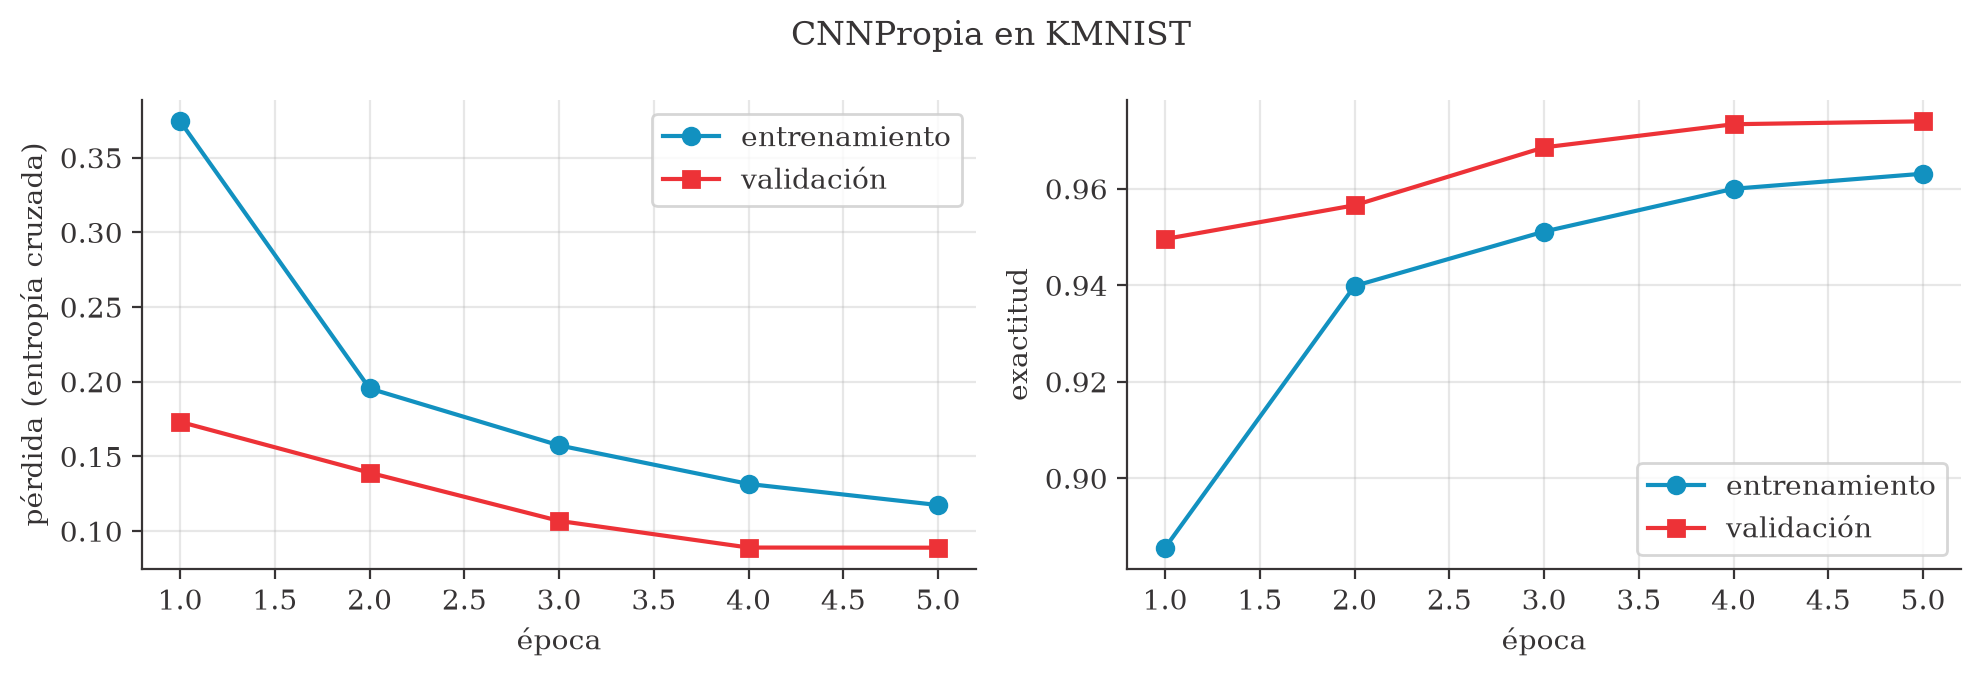
\includegraphics[width=0.60\linewidth]{figuras/f03_curvas_cnnpropia.png}\hfill
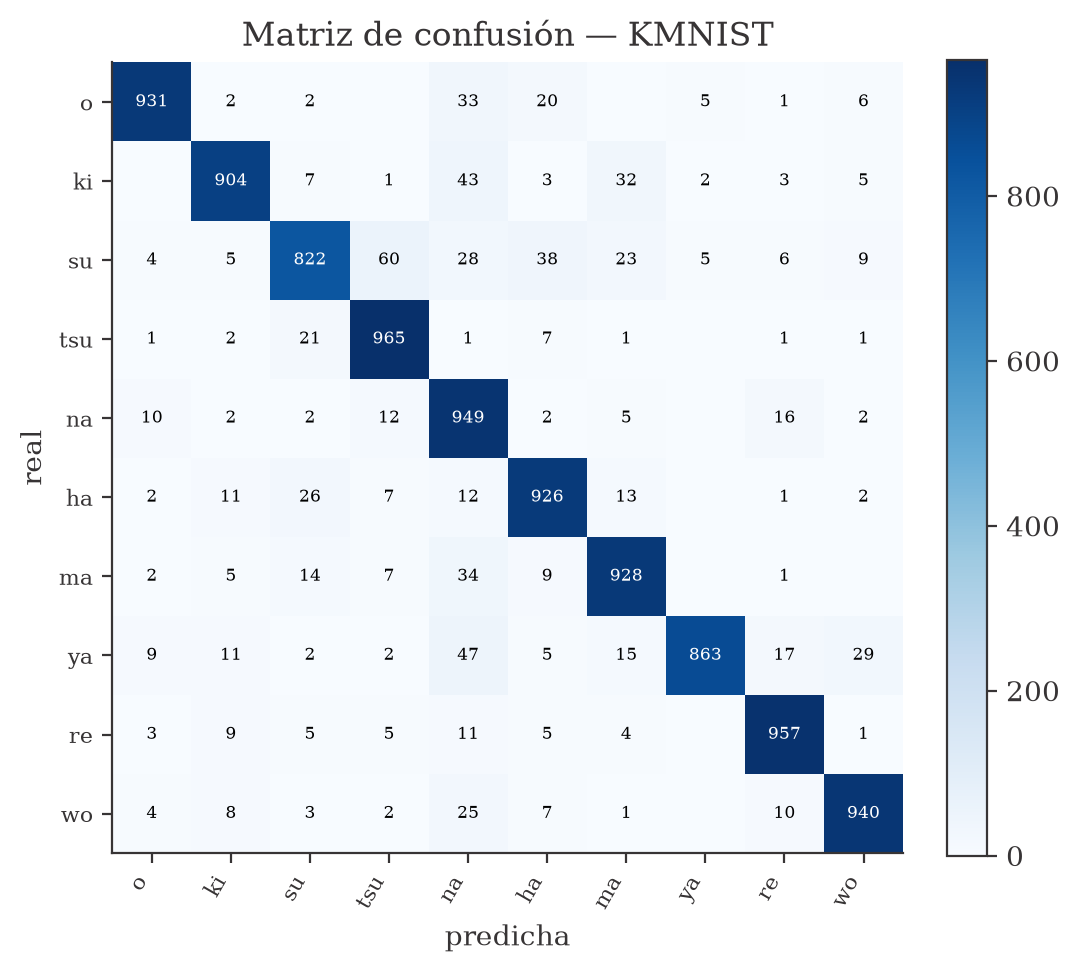
\includegraphics[width=0.36\linewidth]{figuras/f04_matriz_confusion.png}
\caption{Salidas del cuaderno: pérdida y exactitud por época (\cifraepocas{} épocas, 49 s) y matriz de confusión en prueba (\cifraerrTest{} errores de 10\,000).}
\end{figure}

\begin{center}
\begin{tikzpicture}
  \node[hecho, text width=0.9\linewidth, align=left, inner sep=7pt] {%
  \textbf{Resultado.} \texttt{CNNPropia} (20\,586 parámetros) alcanza \textbf{\cifraaccVal\,\%} de exactitud en validación y \textbf{\cifraaccTest\,\%} en prueba. La prueba de KMNIST es más difícil que la
  validación (\cifrabrechaValTest\pts), diferencia que no aparece en MNIST ni en FashionMNIST.};
\end{tikzpicture}
\end{center}

%% ---------------------------------------------------------------------------------------------
\clearpage
\section{Las tres preguntas del taller}

\subsection{¿Por qué cada componente y qué se esperaba de él?}

\begin{table}[H]
\centering\small
\caption{Componentes de la red: qué se esperaba y qué se midió.}
\begin{tabularx}{\linewidth}{@{}l L L l@{}}
\toprule
Componente & Se esperaba & Qué se midió & Resultado \\
\midrule
Convolución & Rasgos locales con pocos parámetros & La CNN del docente (12\,810 parámetros) supera al MLP (101\,770): \cifracnnDocTe\,\% frente a \ciframlpTe\,\% en prueba & Confirmado \\
\textit{BatchNorm} (estabilidad) & Entrenar de forma más estable & Con $\eta=0{,}1$ la misma red llega a \cifralrUno\,\% con \textit{BatchNorm} y a \cifralrSinBnUno\,\% sin ella & Confirmado \\
\textit{BatchNorm} (exactitud) & Mejor exactitud final & Sin ella, la prueba cambia \cifraablBnTe\pts{} (dentro del ruido) & No confirmado \\
\textit{Dropout} & Regularizar la capa final & Sin él: \cifraablDropTe\pts{} en prueba y brecha de \cifraablDropBrecha{} frente a \cifraablBrechaCompleta\pts & Confirmado \\
ReLU y \textit{max-pooling} & No linealidad y tolerar desplazamientos & No se ablacionaron por separado & No evaluado \\
\bottomrule
\end{tabularx}
\end{table}

\subsection{¿Por qué se confunde el par de clases con más errores?}

El par más frecuente es \textbf{\cifraparA{} $\to$ \cifraparB{}} (\cifraparN{} veces; en sentido contrario, \cifraparInv). \textit{su} es la clase más difícil (\cifraclasePeorAcc\,\%). Al mirar imágenes concretas
(figura~\ref{fig:par}), los \textit{su} mal clasificados son casi siempre una \textbf{variante cursiva} distinta de la dominante en la clase y se parecen a grafías de \textit{tsu} bien clasificadas: hay
variación \textbf{dentro} de la clase, no desbalance (las clases tienen entre 5\,450 y 5\,533 imágenes). La confusión es asimétrica, y \textit{na} actúa como ``atractor'' de \textit{ya}, \textit{ki} y \textit{ma}.
Es una lectura visual de las imágenes, no una medición.

\begin{figure}[H]
\centering
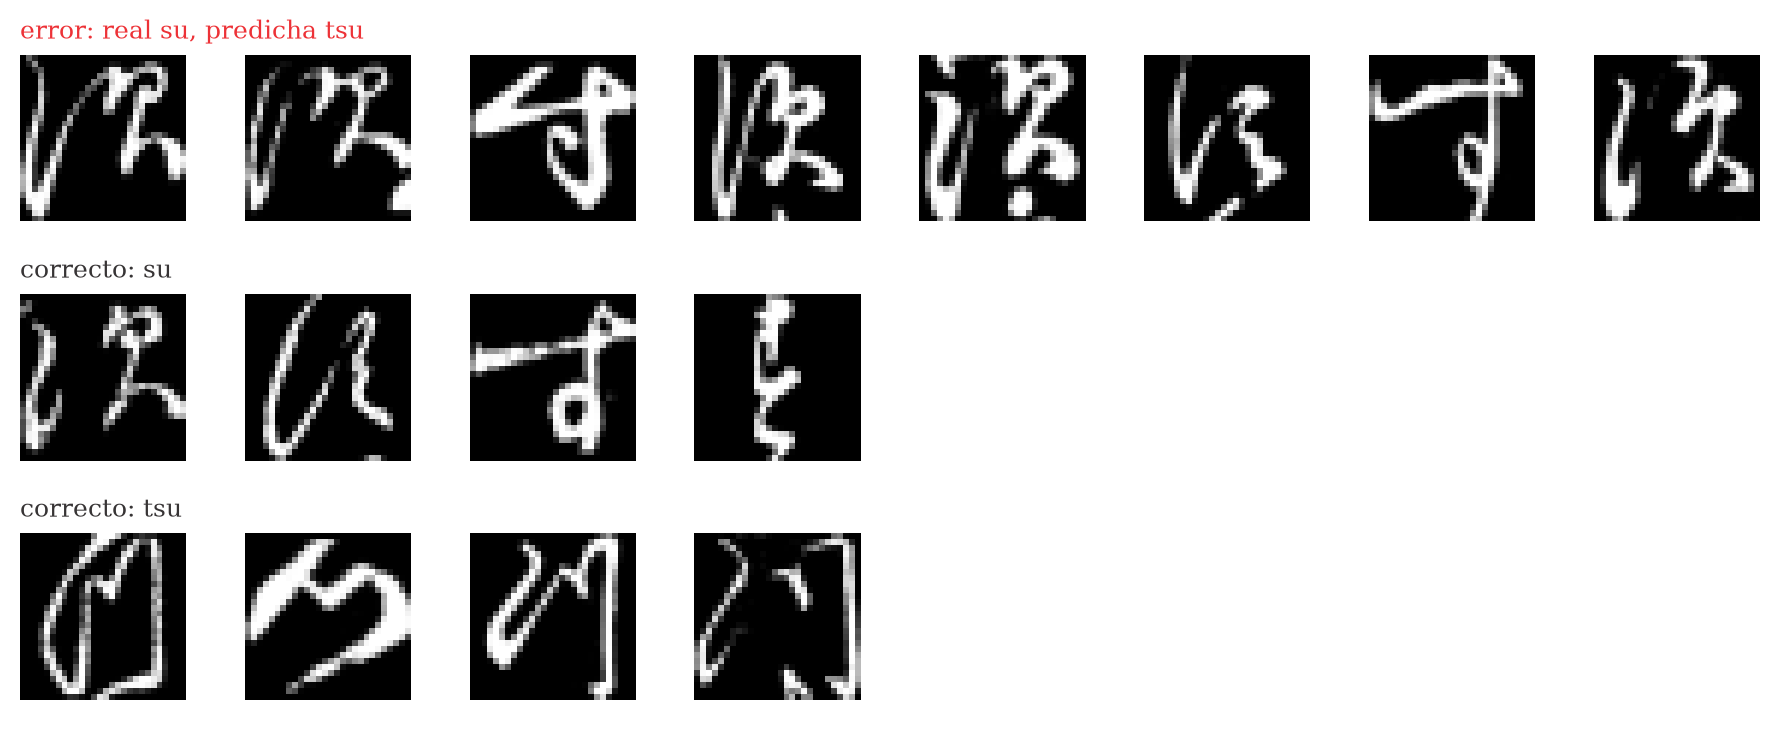
\includegraphics[width=0.85\linewidth]{figuras/f05_par_confundido.png}
\caption{Arriba, errores \textit{su} leído como \textit{tsu}; abajo, aciertos de cada clase para contraste.}\label{fig:par}
\end{figure}

\subsection{¿Mejoró el aumento de datos? ¿Cambió la brecha entre entrenamiento y validación?}

\textbf{No mejoró la exactitud de validación}: con 5 semillas pareadas, el desplazamiento por lote cambia la validación \cifraaugLoteVal\pts{} y el desplazamiento por muestra \cifraaugMuestraVal\pts; en prueba fueron
\cifraaugLoteTe\pts{} y \cifraaugMuestraTe\pts. Con 15 épocas el resultado es el mismo (\cifralargoTeDif\pts{} en prueba). \textbf{La brecha sí cambió}: la diferencia entre exactitud de entrenamiento y de validación
baja de 0,90 a unos 0,2 puntos, es decir, el aumento regulariza, pero esa menor memorización no se traduce en mejor generalización. Posibles razones, no probadas por separado: a 5 épocas casi no hay sobreajuste que corregir;
convolución más \textit{max-pooling} ya tolera desplazamientos pequeños; \texttt{torch.roll} es circular; y los errores de prueba parecen venir de variantes de escritura y no de traslaciones.

\begin{figure}[H]
\centering
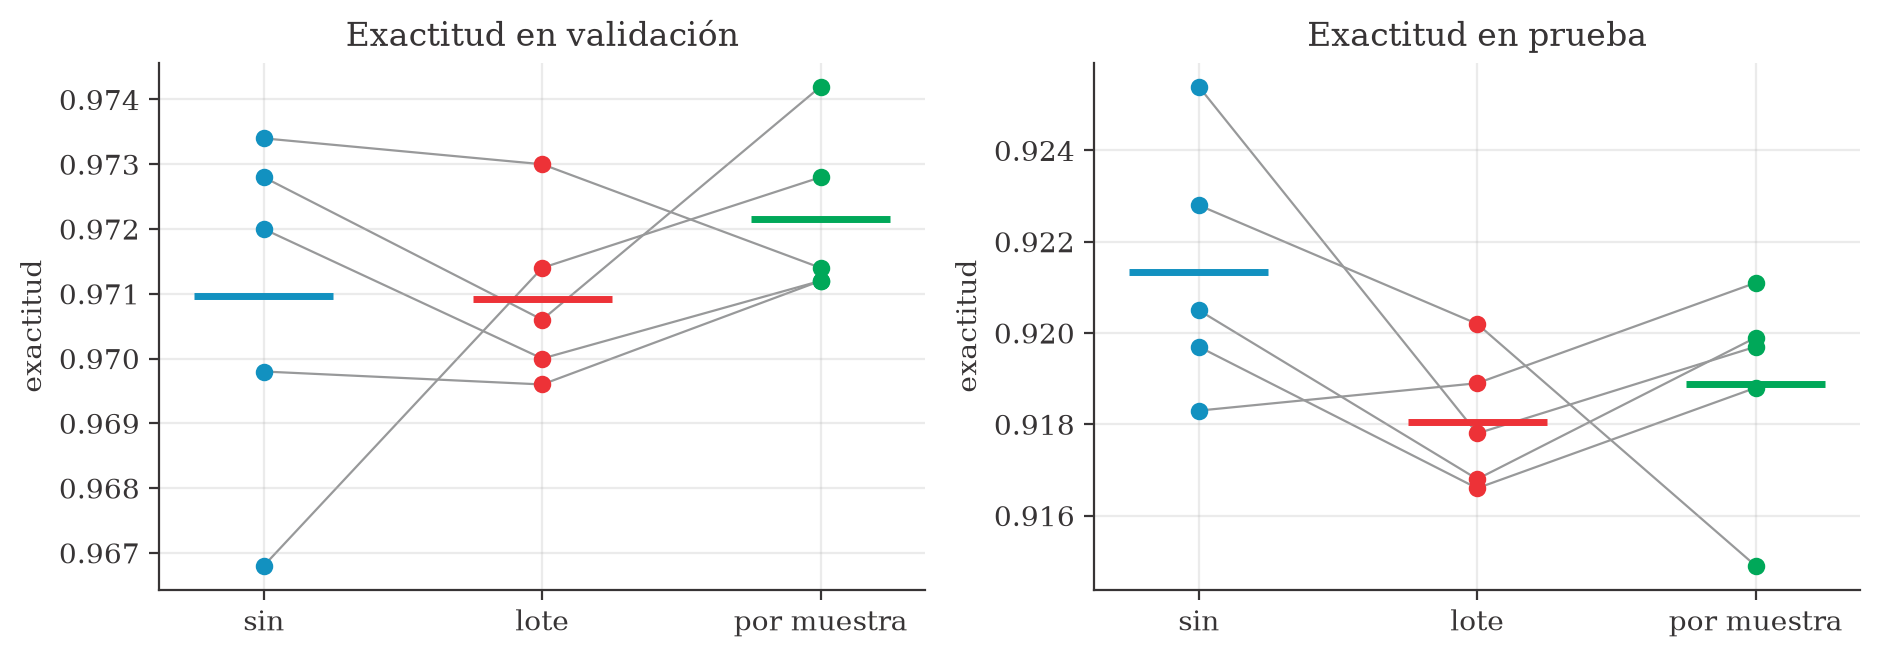
\includegraphics[width=0.92\linewidth]{figuras/f08_aumento_semillas.png}
\caption{Exactitud por semilla (cada punto es una semilla; las líneas grises unen la misma semilla) sin aumento, por lote y por muestra.}
\end{figure}

%% ---------------------------------------------------------------------------------------------
\section{Lectura honesta y reproducibilidad}

\begin{itemize}
  \item \textbf{Validación y prueba no son intercambiables en KMNIST} (\cifraaccVal\,\% frente a \cifraaccTest\,\%). No es un error; la prueba es más difícil y la causa exacta no se midió. Las conclusiones se apoyan en la prueba.
  \item \textbf{Resultado negativo:} el aumento por desplazamiento no mejoró la exactitud; se reporta tal cual. \textbf{Mejora clara:} un tercer bloque convolucional (\cifraablTresTe\pts{} en prueba con 8\,704 parámetros más).
  \item \textbf{Limitaciones:} 3 a 5 semillas, 5 épocas, una arquitectura base y una partición de validación fija; las diferencias de décimas de punto no son concluyentes.
  \item \textbf{Reproducir:} \texttt{make notebook} (aprox.\ 1 h en CPU; reutiliza los resultados guardados) o \texttt{make rapido} (solo los 5 \texttt{TODO}, unos 3 min). Partición con semilla 42; comparaciones con semillas 0 a 4
        (aumento) y 0 a 2 (ablación y bases). El análisis completo está en \texttt{informe/main.pdf}.
\end{itemize}

\end{document}
